\documentclass[../norme-di-progetto.tex]{subfiles}

\begin{document}

\subsection{Descrizione}%
\label{sub:processi_di_supporto/descrizione}

I processi di supporto operano a sostegno degli altri processi con lo scopo di garantire il successo e fornire qualità al progetto.
Essi non esistono autonomamente ma hanno la necessità di appoggiarsi ad altri processi.
ISO 11207:1995 ne distingue otto:

\begin{itemize}
  \item Documentazione
  \item Gestione della configurazione
  \item Accertamento della qualità
  \item Verifica
  \item Validazione
  \item Revisioni congiunte
  \item Verifiche interne
  \item Risoluzione dei problemi.
\end{itemize}

\subsection{Documentazione}%
\label{sub:documentazione}

\subsubsection{Finalità}%
\label{subs:documentazione/finalita}

GruppOne istanzia il processo di documentazione per illustrare in maniera chiara e coerente le attività di processo svolte e i prodotti da esse ottenuti.

\subsubsection{Descrizione}%
\label{subs:documentazione/descrizione}

La documentazione è essenziale durante ogni attività del ciclo di vita del software, essa costituisce un importante mezzo di comunicazione per i membri del team che per il committente.
Si vogliono quindi definire delle norme che possano standardizzare il processo di documentazione e renderlo più accessibile a tutti i componenti del gruppo.

\subsubsection{Implementazione}%
\label{subs:implementazione}

\paragraph{Configurazione}%
\label{par:configurazione}
La configurazione di base comune ai documenti rilevanti è astratta in due file \LaTeX{} che contengono ad esempio\ la struttura e la formattazione che ogni file deve avere.
Si riporta un elenco (non esaustivo) di ciò che è presente nel file di configurazione:

\begin{itemize}
  \item Definizione e decorazione di header e footer.
  \item Definizione dei margini laterali e dell'altezza del footer.
  \item Configurazione dei link.
  \item Dichiarazione di nuovi comandi.
\end{itemize}

\paragraph{Ciclo di vita}%
\label{par:ciclo_di_vita}
Il ciclo di vita di rappresenta gli stadi in cui il documento si può trovare nel corso della sua esistenza. Ne distinguiamo cinque:

\begin{description}
  \item [Creazione del template del documento] un membro del gruppo crea il template del documento il quale conterrà solamente una pagina di frontespizio. Inizialmente sono configurate una serie di impostazioni di base per la formattazione delle pagine grazie all'utilizzo di alcuni package di \LaTeX.
  \item [Scrittura del documento] l'incaricato scrive il documento incrementalmente e lo termina entro la scadenza della \glossario{milestone} fissata.
  \item [Verifica del documento] i \glossario{verificatori} effettuano una revisione del documento segnalando eventuali errori o discordanze che verranno segnalate all'autore del documento che sarà incaricato di correggerli.
  \item [Approvazione del documento] il \glossario{responsabile} di progetto approva il documento.
  \item [Archiviazione] l'amministratore archivia il documento in un repository pubblico su \glossario{GitHub}.
\end{description}

\subsubsection{Struttura}%
\label{subs:struttura}

\paragraph{Frontespizio}%
\label{par:frontespizio}
Il frontespizio è la prima pagina di ogni documento. È diviso in due parti: nella prima è presente l'intestazione contenente logo, nome del gruppo e nome del documento, mentre la seconda consiste di uno schema contenente alcune informazioni essenziali sul documento descritto. In esso compaiono, ordinatamente, dall'alto verso il basso:

\begin{itemize}
  \item Intestazione
        \begin{description}
          \item [Logo] rappresenta il logo del gruppo.
          \item [Nome del gruppo] rappresenta il nome del gruppo.
          \item [Nome del documento] rappresenta nome del documento.
        \end{description}
  \item Schema
        \begin{description}
          \item [Versione] indica la versione attuale del documento (e.g\@. glossario v1.0.0).
          \item [Approvazione] indica chi ha approvato il documento.
          \item [Redazione] indica la lista dei redattori del documento.
          \item [Verifica] indica la lista dei verificatori del documento.
          \item [Stato] indica lo stato attuale in cui si trova il documento.
          \item [Uso] indica l'uso finale del documento (interno o esterno).
          \item [Destinato a] indica lo stato attuale del documento.
          \item [Descrizione] indica una breve descrizione del documento.
        \end{description}
\end{itemize}

\paragraph{Registro delle modifiche}%
\label{par:registro_delle_modifiche}
Il registro delle modifiche ha lo scopo di presentare quali cambiamenti sono stati effettuati e da parte di quale componente del gruppo. Consiste di cinque colonne ed è così articolato:
\begin{description}
  \item [Versione] indica la versione del documento in cui viene realizzata la modifica.
  \item [Data] indica la data di modifica del documento con formato YYYY/MM/DD\@.
  \item [Nominativo] indica nome e cognome del componente del team che ha effettuato la modifica.
  \item [Ruolo] indica il ruolo del componente del team che ha realizzato la modifica.
  \item [Descrizione] indica il tipo e il luogo in cui è avvenuta la modifica.
\end{description}

\paragraph{Indice}%
\label{par:indice}
L'indice presenta presenta l'elenco, accompagnato dal numero di pagina, delle sezioni e dei paragrafi di cui è composto il documento.
GruppOne ha deciso di utilizzare la tipica suddivisione del testo offerta da \LaTeX{} che distingue cinque diversi blocchi testuali:
\begin{itemize}
  \item Sezioni
  \item Sottosezioni
  \item Sotto-sottosezioni
  \item Paragrafi
  \item Sottoparagrafi.
\end{itemize}

Ogni blocco testuale ha un numero identificativo univoco la cui lunghezza dipende dal grado di annidamento del blocco ed è predefinita in \LaTeX{} (e.g.:\ la sezione Introduzione è indicata con 1, la relativa sottosezione quattro è indicata con 1.4 e i capitoli contenuti in quella sottosezione sono indicati con 1.4.1 e 1.4.2).
Ogni blocco testuale si identifica mediante una \glossario{label} univoca, utile a creare riferimenti interni al documento.

Ogni riga dell'indice contiene il numero di pagina in cui si trova la sezione o il paragrafo a cui si riferisce e, cliccando sul nome del blocco, è possibile raggiungerlo direttamente.

\paragraph{Contenuto}%
\label{par:contenuto}
Le pagine di contenuto sono suddivise in tre parti, dall'alto verso il basso:
\begin{description}
  \item [Header] contiene sinistra il logo del gruppo, a destra il nome del documento.
  \item [Contenuto] contiene il testo del documento.
  \item [Footer] contiene l'indicazione della pagina attuale rispetto il totale (e.g 1 di 6).
\end{description}

\paragraph{Norme per la redazione dei documenti}%
\label{par:norme_per_la_redazione_dei_documenti}

\subparagraph{Stile del testo}%
\label{subp:stile_del_testo}
In questo paragrafo GruppOne definisce le norme che uniformano lo stile di scrittura dei documenti:
\begin{description}
  \item [Verbi in forma attiva] i verbi devono essere in forma attiva e al tempo presente indicativo o passato prossimo. È ammesso l'uso del futuro per esprimere azioni che devono ancora avvenire.
  \item [Struttura del testo chiara] la suddivisione del testo in sezioni, sottosezioni e paragrafi aiuta la coerenza e la coesione.
  \item [Frasi brevi e poco complesse] i periodi devono essere il più possibile semplici per non generare incomprensioni.
  \item [Uso degli elenchi puntati] per evitare lunghe digressioni ed eccessiva verbosità si vogliono utilizzare gli elenchi puntati laddove è possibile.
  \item [Brevi blocchi testuali] si preferisce l'utilizzo di brevi paragrafi.
  \item [Termini di glossario in maiuscolo] il testo è scritto in minuscolo. I termini di glossario, invece, sono indicati in maiuscolo con una g a pedice nel nome. Questa regola vale per la prima occorrenza di ogni termine di glossario.
\end{description}

\subparagraph{Elenchi }%
\label{subp:elenchi}
Gli elenchi sono un ottimo mezzo per la scrittura di documentazione. Essi permettono di riordinare il testo e di organizzare una serie di elementi correlati, pertanto, in questo paragrafo, si stabiliscono le norme per il loro corretto uso:

\begin{enumerate}
  \item Per indicare gli elementi di un elenco puntato non innestato utilizziamo il simbolo •. Gli elementi innestati sono preceduti da -.
  \item Ogni elemento di elenco puntato inizia con una lettera maiuscola.
  \item Se un elenco ha elementi composti da etichetta e descrizione, l'etichetta deve essere scritta in grassetto e la descrizione va inserita dopo i due punti.
  \item Gli elenchi puntati semplici non hanno bisogno di punti fermi per terminare la frase. Gli elenchi puntati complessi, che possono essere formati da lunghi periodi, necessitano di un punto al termine della frase.
  \item L'ultimo elemento dell'elenco deve comunque avere obbligatoriamente un punto al termine della frase.
\end{enumerate}

\subparagraph{Nomi dei file}%
\label{nomi_dei_file}
Per identificare i file memorizzati nel repository si seguono le seguenti convenzioni:

\begin{itemize}
  \item I nomi dei file devono essere in minuscolo e ignorare eventuali accenti o apostrofi.
  \item Le parole contenute nei nomi di file composti devono essere separate da -.
\end{itemize}

Analisi dei requisiti sarà quindi salvato come analisi-dei-requisiti, mentre Norme di progetto come norme-di-progetto.

\subparagraph{Sigle}%
\label{subp:sigle}
Si elencano una serie di sigle che possono essere utilizzate nei documenti. Si accompagna ad ognuna di esse il relativo significato:

\begin{itemize}
  \item sigle per identificare le revisioni
        \begin{description}
          \item [RR] revisione dei requisiti
          \item [RP] revisione di progettazione
          \item [RQ] revisione di qualifica
          \item [RA] revisione di accettazione.
        \end{description}
  \item sigle per identificare i documenti
        \begin{description}
          \item [AdR] analisi dei requisiti
          \item [NdP] norme di progetto
          \item [PdQ] piano di qualifica
          \item [PdP] piano di progetto
          \item [MU] manuale utente
          \item [MS] manuale sviluppatore
          \item [G] glossario
          \item [V] verbali.
        \end{description}
  \item sigle per identificare i ruoli
        \begin{description}
          \item [Re] responsabile
          \item [Am] amministratore
          \item [An] analista
          \item [Pgt] progettista
          \item [Pgr] programmatore
          \item [Ve] verificatore.
        \end{description}
\end{itemize}

\subparagraph{Convenzioni comuni}%
\label{subp:convenzioni_comuni}
Per la scrittura delle date si fa uso della seguente convenzione:
\begin{center}
  \textbf{YYYY-MM-DD}
\end{center}
Ad esempio 15 Novembre 2019 si scrive 2019--11--15.

\subparagraph{Immagini}%
\label{subp:immagini}
Le immagini si devono utilizzare per apportare un valore aggiunto a ciò che si sta descrivendo o per dare una rappresentazione grafica di ciò che si sta presentando.
Immagini con funzione puramente estetica non sono pertanto ammesse, ad eccezione di quanto definito nel template comune.
Tutte le immagini devono essere inoltre centrate all'interno della pagina e munite di una breve didascalia così formata:
\begin{center}
  \textbf{Figura x: breve descrizione dell'immagine}
\end{center}
dove x indica la numerazione delle immagini (e.g.:\ figura 1, figura 2, figura 3).

\subparagraph{Tabelle}%
\label{subp:tabelle}
L'uso di tabelle è consigliato solo quando strettamente necessario. La rappresentazione dei dati in forma tabellare è obbligatoria solo nel momento in cui risulti molto difficile organizzare informazioni aventi una struttura complessa. È obbligatorio l'uso di colori che abbiano un elevato contrasto al fine di promuovere la leggibilità. Inoltre, non devono essere eccessivamente lunghe altrimenti risultano dispersive.

\subsubsection{Produzione}%
\label{subs:produzione}

\paragraph{Suddivisione dei documenti}%
\label{par:suddivisione_dei_documenti}
I documenti utilizzano la struttura a \glossario{subfiles} offerta da \LaTeX.
La struttura di base del documento è definita nel file che porta il nome del documento.
La cartella components, che è unica per ogni documento, contiene un file per la definizione di ogni sezione. In ogni sezione si definiscono poi le relative sottosezioni, paragrafi e sottoparagrafi.

Ad esempio, il file norme di progetto ha la seguente struttura:

\begin{itemize}
  \item[] \ldots
  \item[] /interni/
        \begin{itemize}
          \item[] norme-di-progetto/
                \begin{itemize}
                  \item[] components/
                        \begin{itemize}
                          \item[] introduzione.tex
                          \item[] \ldots
                        \end{itemize}
                  \item[] norme-di-progetto.tex
                \end{itemize}
          \item[] \ldots
        \end{itemize}
  \item[] \ldots
\end{itemize}

\subparagraph{Interni}%
\label{subp:suddivisione_dei_documenti/interni}
I documenti interni sono destinati alla comunicazione tra i componenti di GruppOne. Appartengono a tale categoria:

\begin{itemize}
  \item Verbali interni
  \item Studio di fattibilità
  \item Norme di progetto.
\end{itemize}

\subparagraph{Esterni}%
\label{subp:suddivisione_dei_documenti/esterni}
I documenti esterni sono destinati al committente. Appartengono a tale categoria:

\begin{itemize}
  \item Analisi dei requisiti
  \item Piano di progetto
  \item Piano di qualifica.
\end{itemize}

\subparagraph{Verbali}%
\label{subp:verbali}
I verbali contengono un riassunto degli incontri di GruppOne.
Se qualche componente del gruppo non fosse presente ad un incontro verbale, è necessario che prenda visione del relativo verbale, in modo da informarsi sugli argomenti discussi alla riunione in cui era assente.
I verbali si distinguono in interni ed esterni. Ogni verbale è contraddistinto da un nome così strutturato:
\begin{center}
  \textbf{verbaleYYYY-MM-DD.tex}
\end{center}
I verbali sono così costituiti:

\begin{description}
  \item [Titolo] il titolo indica che il documento in questione è un verbale e mostra la data di redazione.
  \item [Schema] lo schema contiene le informazioni basilari relative al documento. È identico allo schema degli altri documenti, spiegato nella sezione~\ref{par:frontespizio}.
  \item [Registro delle modifiche] il registro delle modifiche ha la struttura di quello presentato in~\ref{par:registro_delle_modifiche}.
  \item [Ordine del giorno] l'ordine del giorno consiste in un elenco puntato degli argomenti che saranno trattati nel verbale.
  \item [Sezioni] Ogni sezione del documento sviluppa un elemento dell'ordine del giorno.
  \item [Registro delle decisioni] il registro delle decisioni indica le decisioni prese sulla base degli argomenti discussi nell'ordine del giorno.
\end{description}

\subsubsection{Strumenti}

\paragraph{\LaTeX}%
\label{par:LaTeX}
\LaTeX{} (versione \href{https://texfaq.org/FAQ-latex2e}{\LaTeX2e}) è il linguaggio di markup utilizzato da GruppOne per la stesura dei documenti.
Ogni componente del gruppo ha installato sul proprio sistema una distribuzione di \TeX{}/\LaTeX{} a piacere che includesse Lua\TeX{} e ne esponesse sul \verb|PATH| l'eseguibile.

Ognuno ha inoltre aggiunto un'estensione per il proprio Code Editor preferito che consentisse di facilitare la corretta esecuzione del processo di build dei file *.tex.

Questa avviene attraverso il comando:

\begin{minted}{bash}
  lualatex `
    --interaction=nonstopmode `
    --c-style-errors `
    --shell-escape `
    <file-to-build>
\end{minted}

Da eseguire due volte per permettere a \LaTeX{} di recuperare i riferimenti corretti e ad es\@. il numero totale di pagine.

È inoltre necessario avere disponibile sul proprio sistema \href{https://pygments.org/}{Pygments}, un package di python richiesto dal package di \LaTeX{} \href{https://ctan.org/pkg/minted?lang=en}{minted}, che permette di evidenziare la sintassi degli \glossario{snippet} di codice presenti nel documento.

\subsubsection{Metriche}%
\label{subs:documentazione/metriche}

% TODO sposta metriche qui

% subs:metriche (end)

% TODO finire di scrivere gestione della config
\subsection{Gestione della configurazione}%
\label{sub:gestione_della_configurazione}

\subsubsection{Finalità}%
\label{subs:gestione_della_configurazione/finalita}

GruppOne istanzia il processo di gestione della configurazione per:
\begin{itemize}
  \item Assicurare completezza e correttezza del prodotto.
  \item Gestire al meglio il lavoro di gruppo.
  \item Identificare procedure per l'organizzazione, gestione e rilascio del prodotto.
  \item Conservare documentazione e software in un luogo accessibile e compatibile con la licenza richiesta dal prodotto.
\end{itemize}

\subsubsection{Gestione del versionamento}%
\label{subs:gestione_del_versionamento}

\paragraph{Repository}%
\label{par:repository}

\paragraph{Struttura dei commit}%
\label{par:struttura_dei_commit}

\subsubsection{Strumenti}%
\label{subs:gestione_della_configurazione/strumenti}

\subsection{Accertamento della qualità}%
\label{subs:accertamento_della_qualita}

\subsubsection{Finalità}%
\label{subs:accertamento_della_qualita/finalita}

GruppOne istanzia il processo di accertamento della qualità per garantire qualità di processo e di prodotto.
Gli esiti dei processi di verifica e validazione saranno indispensabili nello svolgimento del processo di accertamento della qualità.

\subsubsection{Descrizione}%
\label{subs:accertamento_della_qualita/descrizione}

Il processo di accertamento della qualità garantisce che i prodotti e i processi del ciclo di vita del software rispettino i requisiti prestabiliti e che aderiscano ai piani esecutivi prefissati. Le metriche e gli strumenti per valutare la qualità sono presentati nel \glossario{piano di qualifica}.

\subsubsection{Attività}%
\label{subs:accertamento_della_qualita/attivita}

Le principali attività coinvolte nel processo di accertamento della qualità sono:

\begin{description}
  \item [Pianificazione] si cercano le metodologie, le procedure, gli strumenti le attività offerte da altri processi di supporto per organizzare le pianificazione della qualità.
  \item [Implementazione] si utilizza ciò che si è individuato al punto precedente per effettuare controlli di qualità sui processi e sui prodotti in atto.
  \item [Documentazione dei risultati] i risultati dei controlli di qualità dovrebbero essere poi documentati.
\end{description}

\paragraph{Accertamento qualità di prodotto}%
\label{par:accertamento_qualita_di_prodotto}
L'attività di accertamento della qualità di prodotto assicura la qualità dei prodotti realizzati e promuove controlli continui che possano prevenire danni irreparabili al termine del progetto. È fortemente dipendente dalla qualità di processo: da processi privi di qualità, infatti, non è possibile ottenere buoni prodotti.

\paragraph{Accertamento qualità di processo}%
\label{par:accertamento_qualita_di_processo}
L'attività di accertamento della qualità di processo monitora i processi istanziati. Per avere un sistema di accertamento della qualità di processo che funzioni è necessario che:

\begin{itemize}
  \item Si individuino i processi da controllare.
  \item Si stabiliscano le metriche di valutazione del processo.
  \item Si eseguano accertamenti continui sui processi scelti.
  \item In base ai risultati ottenuti, si ricerchi un miglioramento dei processi.
\end{itemize}

\subparagraph{PDCA}%
\label{subp:PDCA}
Il ciclo di Deming o ciclo PDCA è un processo iterativo per il monitoraggio e il miglioramento di processo. Sfrutta la ripetizione di quattro attività:

\begin{description}
  \item [Plan] definisce gli obiettivi, le attività e i processi necessari per raggiungere i risultati attesi.
  \item [Do] esegue ciò che è stato definito nella fase di pianificazione.
  \item [Check] verifica gli esiti dei processi.
  \item [Act] esegue azioni correttive per migliorare la qualità dei processi.
\end{description}
\begin{figure}[H]
  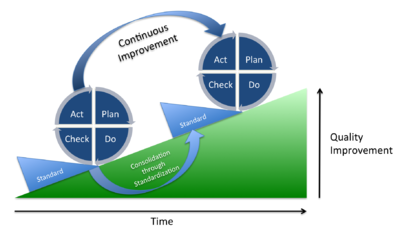
\includegraphics[width=8cm]{PDCA-process.png}
  \centering
  \caption{ciclo di Deming o PDCA.}
\end{figure}

\subsection{Verifica}%
\label{sub:verifica}

\subsubsection{Finalità}%
\label{subs:verifica/finalita}

GruppOne istanzia il processo di verifica per certificare che il susseguirsi di attività diverse non comporti l'introduzione di errori nei prodotti intermedi.
Si deve verificare qualsiasi prodotto intermedio, pertanto sia documentazione che codice sono soggetti a verifica.

\subsubsection{Descrizione}%
\label{subs:verifica/descrizione}


Il processo di verifica è il processo che controlla e garantisce che i prodotti di una determinata attività soddisfino i requisiti e le condizioni che quel prodotto deve avere. Il processo di verifica si integra in toto con gli altri processi, in particolare con quello di sviluppo, e offre attività di revisione, analisi e test. È composto da due attività:

\begin{itemize}
  \item Implementazione di processo
  \item Verifica.
\end{itemize}

\paragraph{Analisi statica}%
\label{par:analisi_statica}
L'analisi statica consiste nell'insieme delle buone pratiche che valutano un componente del sistema sulla base della sua forma, struttura e contenuto.
L'analisi statica quindi definisce una serie di regole a cui tutti i prodotti intermedi del ciclo di vita del software devono attenersi. Esistono due tipi di analisi statica:
\begin{description}
  \item [Walkthrough] La tecnica walkthrough esegue una verifica a largo spettro del prodotto. Si articola nelle seguenti attività:
        \begin{itemize}
          \item Pianificazione di cosa è necessario monitorare.
          \item Lettura dell'oggetto di verifica da parte di più membri del team.
          \item Discussione dei difetti individuati da tutti i componenti del team.
          \item Correzione concordata degli errori trovati.
        \end{itemize}
  \item [Inspection] la tecnica inspection esegue una verifica mirata del prodotto. Si articola nelle seguenti attività:
        \begin{itemize}
          \item Pianificazione di cosa è necessario monitorare.
          \item Costruzione di una checklist di controllo.
          \item Lettura dell'oggetto di verifica sulla base delle metriche definite nella lista di controllo.
          \item Correzione degli errori trovati.
        \end{itemize}
\end{description}
GruppOne predilige la tecnica inspection pertanto si impegna a fornire una checklist dei controlli da effettuare sui documenti e sul software.

\subparagraph{Analisi statica dei documenti}%
\label{subp:analisi_statica_dei_documenti}
Di seguito si riporta una checklist da seguire per effettuare l'analisi statica dei documenti:

\begin{description}
  \item [Errori di ortografia] si devono individuare errori di punteggiatura e ortografia.
  \item [Errori nei verbi] si deve controllare che tutti i verbi siano in forma attiva.
  \item [Errori di sintassi] si deve verificare che non ci siano paragrafi di lunghezza eccessiva e che le frasi siano il più brevi possibile.
  \item [Errori negli elenchi puntati] si deve controllare che ogni elemento degli elenchi puntati inizi con la lettera maiuscola e che vengano rispettate le regole definite in~\ref{subp:elenchi}.
  \item [Errori nella strutturazione del documento] si deve verificare che tutti i paragrafi si trovino nella sezione corretta, che le sezioni siano ben strutturate e che i titoli siano significativi.
\end{description}

Sarà compito dei verificatori attenersi alla checklist definita in~\ref{subp:analisi_statica_dei_documenti} per le attività di verifica.

\paragraph{Analisi dinamica del codice}%
\label{par:analisi_dinamica_del_codice}
L'analisi dinamica del codice necessita che l'oggetto di verifica sia in esecuzione.
Essa cerca di dimostrare che il programma svolge i compiti per il quale è stato realizzato e identifica gli errori prima che il software sia messo in uso.
Si realizza attraverso la creazione e l'esecuzione di test che producono deterministicamente un risultato da confrontare con un valore atteso.
Il numero di test è chiaramente finito e quindi non sarà possibile provare tutte le esecuzioni possibili.
Per questo motivo bisogna produrre dei test sensati.
Un test, affinché sia definito come tale, deve avere delle precise caratteristiche:

\begin{itemize}
  \item Velocità
  \item Ripetibilità
  \item Bassa interazione umana.
\end{itemize}

\subparagraph{Copertura dei test}%
\label{subp:copertura_dei_test}
Per ogni tipo di test è necessario fornire la sua copertura.
Essa è un valore percentuale e indica quanti \glossario{statement} i test hanno eseguito rispetto al totale.
Più la copertura è alta meglio è, tuttavia una copertura del 100 \% non dà in alcun modo la certezza di essere in assenza di difetti.
Il capitolato di Stalker richiede una copertura dei test pari almeno all' 80 \%, correlata di report.

\subparagraph{Test di unità}%
\label{subp:test_di_unita}
Il software è un insieme di componenti. Per effettuare verifica del software è necessario adottare un approccio \glossario{bottom-up} che deve necessariamente occuparsi di controllare anzitutto che le unità su cui è costruito il software siano corrette. I test di unità, quindi, servono a testare i moduli elementari del software.

\subparagraph{Test di integrazione}%
\label{subp:test_di_integrazione}
I test di integrazione si occupano di verificare l'interazione tra le sottocomponenti del sistema.
Essi suppongono che i test di unità siano già stati eseguiti e abbiano dato esito positivo.
Lo scopo dei test di integrazione è quello di dimostrare che le interfacce delle componenti del software si comportino in conformità alle specifiche richieste.

\subparagraph{Test di sistema}%
\label{test_di_sistema}
I test di sistema si possono iniziare solo nel momento in cui i test di integrazione abbiano dato esito positivo.
Essi verificano il comportamento generale del software rispetto ai requisiti.
Durante i test di sistema si esercitano le funzionalità di alcune componenti del software che sono fortemente dipendenti da altri moduli del sistema.

\subparagraph{Test di regressione}%
\label{test_di_regressione}
I test di regressione servono per accertare che le modifiche apportate non comportino altri errori nel software: consistono nella ripetizione selettiva di test di unità, integrazione, test di sistema.

\subparagraph{Test di accettazione}%
\label{test_di_accettazione}
I test di accettazione verificano il completo soddisfacimento dei requisiti utente.
Sono eseguiti in collaborazione con il committente.

\paragraph{Metriche}%
\label{par:metriche}

\subparagraph{Denominazione}%
\label{subp:denominazione}
Le metriche sono essenziali per avere una misura oggettiva di qualità del nostro prodotto.
Per tale ragione per la definizione delle metriche di qualità è necessario identificare una denominazione comune.
Ogni metrica avrà la seguente struttura:
\begin{center}
  \textbf{M[Tipo][Codice]}
\end{center}
\begin{description}
  \item [Tipo] indica il tipo di metrica. Può essere:
        \begin{itemize}
          \item PS- metrica di processo.
          \item PR- metrica di prodotto.
        \end{itemize}
  \item [Codice] un codice identificativo univoco a tre cifre che rappresenta la metrica.
\end{description}


\subparagraph{MPS001-Indice di Gulpease}%
\label{subp:MPS001-indice_di_Gulpease}

L'indice di Gulpease è un indice che valuta la leggibilità di un testo scritto in lingua italiana. Ha il vantaggio principale di utilizzare la lunghezza delle parole in lettere invece che sillabe. La formula per il calcolo è la seguente:
\[
  89 +\frac{300\cdot nf-10\cdot nl}{np}
\]
dove:
\begin{description}
  \item [nf] indica il numero delle frasi.
  \item [nl] indica il numero delle lettere.
  \item [np] indica il numero di parole.
\end{description}
I risultati sono compresi tra 0 e 100 dove 0 indica la leggibilità minima mentre 100 quella massima. In genere l'indice dice che:
\begin{itemize}
  \item Un testo con indice inferiore a 80 è difficile per chi ha la licenza elementare.
  \item Un testo con indice inferiore a 60 è difficile per chi la licenza media.
  \item Un testo con indice inferiore a 40 è difficile per chi ha il diploma di scuola superiore.
\end{itemize}
\subparagraph{MPS002-Indice di Gunning Fog}%
\label{subp:MPS002-indice_di_Gunning_Fog}

L'indice di Gunning Fog è un indice progettato per misurare la facilità di lettura e la comprensione del testo. La formula per il calcolo è la seguente:
\[
  0.4\cdot((\frac{np}{nf})+100\cdot(\frac{npc}{np}))
\]
dove:
\begin{description}
  \item [np] indica il numero di parole.
  \item [nf] indica il numero di frasi.
  \item [npc] indica il numero di parole complesse, dove per complesse si intendono le parole con più di tre sillabe escluse:
        \begin{itemize}
          \item Parole composte da due parole di una o due sillabe.
          \item Nomi propri.
          \item Verbi di due sillabe che coniugati diventano di tre sillabe o più.
          \item Avverbi in -ente di parole di due sillabe.
        \end{itemize}
\end{description}
Il numero risultante indica il numero di anni minimi di educazione formale necessari a comprendere il testo. Ad esempio se l'indice vale 17 vuol dire che il testo potrà essere letto facilmente da una persona con licenza di scuola media.

\subparagraph{MPS003-Correttezza ortografica}%
\label{subp:MPS003-correttezza_ortografica}

L'indice di correttezza ortografica indica la correttezza del testo.
Esso misura il numero di errori ortografici presenti.
Ogni componente del gruppo ha un estensione per il proprio code editor (per vscode consigliamo l'estensione \href{https://marketplace.visualstudio.com/items?itemName=ban.spellright}{Spell Right}, che si basa sul dizionario di sistema).

\subparagraph{MPS004-Requisiti obbligatori soddisfatti}%
\label{subp:MPS004-requisiti_obbligatori_soddisfatti}

La metrica MPS004 indica la percentuale di requisiti obbligatori soddisfatti sul numero totale di requisiti obbligatori. La formula è la seguente:
\[
  \frac{requisiti\ obbligatori\ soddisfatti}{requisiti\ obbligatori\ totali}\cdot 100
\]

\subparagraph{MPS005-Varianza dei costi}%
\label{subp:MPS005-varianza_dei_costi}

La metrica MPS005 misura se il costo effettivamente maturato al momento del calcolo dell'indice sia in linea con quanto pianificato. Si calcola:
\[
  BCWP-ACWP
\]
dove:
\begin{description}
  \item [BCWP] misura il costo del lavoro svolto alla data attuale.
  \item [ACWP] indica il costo sostenuto alla data corrente.
\end{description}

\subparagraph{MPS006-Varianza rispetto allo schedule}%
\label{subp:MPS006-varianza_rispetto_allo_schedule}

La metrica misura se si è in anticipo o in ritardo rispetto rispetto allo schedule delle attività di progetto pianificate nella baseline. Si calcola:
\[
  BCWP - BCWS
\]
dove:
\begin{description}
  \item [BCWP] misura il costo del lavoro svolto alla data attuale.
  \item [BCWS] indica il budget previsto per la realizzazione dell'intero progetto.
\end{description}
Il numero risultante indica:
\begin{itemize}
  \item Una varianza di schedule pari a 0 indica che si sta rispettando la pianificazione.
  \item Una varianza di schedule inferiore a 0 indica che si è in ritardo rispetto alla pianificazione.
  \item Una varianza di schedule superiore a 0 indica che si è in anticipo rispetto alla pianificazione.
\end{itemize}

\subparagraph{MPS007-Rischi incontrati e non preventivati}%
\label{subp:MPS007-rischi_incontrati_e_non_preventivati}

La metrica misura il numero di rischi incontrati che non sono stati preventivati nell'analisi dei rischi del \textit{Piano di progetto}. Un valore maggiore di 0 indica una analisi dei rischi effettuata in maniera non ottimale.

% TODO parlare delle GitHub action?
\paragraph{Strumenti}%
\label{par:verifica/descrizione/strumenti}

\subparagraph{Linter}%
\label{subp:linter}

% Un linter è uno strumento che analizza il codice sorgente per determinare errori di programmazione o costrutti sintattici ritenuti non corretti
Per la verifica del codice ogni componente ha installato sulla propria macchina un \glossario{linter}.
Abbiamo deciso di utilizzare \href{https://www.nongnu.org/chktex/}{Chk\TeX}, che è incluso nella maggior parte delle distribuzioni \LaTeX{} così come nell'estensione di Visual Studio Code che utilizziamo, ed è facilmente configurabile per le nostre necessità.

\subparagraph{Code owners}%
\label{subp:code_owners}

Abbiamo adattato alle nostre necessità la feature \href{https://help.github.com/en/github/creating-cloning-and-archiving-repositories/about-code-owners}{Code Owners} offerta da GitHub.
All'interno del file \verb|CODEOWNERS| posizionato nella cartella \verb|.github| nella radice del repository, abbiamo definito due code owner per ogni documento di progetto.
Ogni volta che viene aperta una \glossario{Pull Request} che modifica alcuni file, i rispettivi code owner vengono notificati automaticamente e viene loro richiesta una verifica dei cambiamenti effettuati.

% TODO sposta in pdq
% L'integrazione delle modifiche nella branch di default del repository è condizionata al superamento di queste verifiche.

\subsection{Validazione}%
\label{sub:validazione}

\subsubsection{Finalità}%
\label{subs:validazione/finalita}

GruppOne istanzia il processo di validazione per assicurarsi che il prodotto finale realizzato soddisfi pienamente le attese del committente.

\subsubsection{Descrizione}%
\label{subs:validazione/descrizione}

Dovendo verificare se il prodotto finale soddisfa i requisiti, anche il processo di validazione fa uso dell'analisi dinamica del codice e quindi di test ad hoc per dimostrare la correttezza del prodotto.

\subsubsection{Piano di validazione}%
\label{subs:piano_di_validazione}

Il piano di validazione comprende tutte le attività del processo di validazione:

\begin{itemize}
  \item Scelta dell'oggetto di validazione.
  \item Decisione dei compiti da eseguire per realizzare la validazione.
  \item Determinazione delle risorse e delle responsabilità.
  \item Procedure per fornire al cliente i report di validazione.
\end{itemize}

\subsubsection{Metriche}%
\label{subs:validazione/metriche}

% TODO scrivi metriche

% subs:metriche (end)

\subsection{Processo di risoluzione dei problemi}%
\label{sub:processo_di_risoluzione_dei_problemi}

\subsubsection{Finalità}%
\label{subs:processo_di_risoluzione_dei_problemi/finalita}

GruppOne istanzia il processo di risoluzione dei problemi per affrontare sia i rischi che si sono manifestati concretamente che quelli non previsti, cercando di ridurre al minimo questi ultimi attraverso analisi e gestione dei rischi.

\subsubsection{Descrizione}%
\label{subs:processo_di_risoluzione_dei_problemi/descrizione}

Per effettuare il tracciamento dei problemi riscontrati utilizziamo gli issue di GitHub come \glossario{ticket}, facendo attenzione a utilizzare i label corretti (e.g\@. bug, invalid) in modo da distinguerli ed effettuarne una prioritizzazione adeguata.

L'attività di risoluzione dei problemi verrà istanziata ove necessario, identificando chiaramente chi ne è responsabile, che dovrà provvedere a riportare nel ticket corrispondente la soluzione applicata.

\subsubsection{Metriche}%
\label{subs:processo_di_risoluzione_dei_problemi/metriche}

% TODO scrivi metriche

% sub:risoluzione_dei_problemi (end)

\end{document}
